\chapter{File di Esempio}
   Questo 
   file vuole solo essere un esempio di
   \LaTeX2, guardate il sorgente se volete capire come \`e fatto.

   Se inoltre volete capire come mai per scrivere ``è'' ho usato quello strano
   \emph{accrocchio} passate alla sezione~\ref{accenti}, notate inoltre
   che andare a capo due volte di seguito mi genera un nuovo paragrafo.
   Notate che l'\emph{indentatura} che sto usando \`e solo per semplicit\`a.

\section{Grassetto, Italico e amenit\`a varie}
   \`E banale ottenerli (a differenza della ``e'' maiuscola e
   accentata quando usate qualcosa di diverso dal \LaTeX2),
   gi\`a che ci siamo potete anche vedere come si
   ottiene una lista e un nota a pi\`e di pagina:
   \begin{itemize}
   \item \textbf{Grassetto}
   \item \emph{Italico}
   \item \textsc{Maiuscoletto}
   \item \texttt{Macchina da Scrivere}\footnote{In genere \`e conveniente non
                 abusare troppo di questo, visto che \`e gestito male nei rientri a capo.}
   \end{itemize}
\section{Tabelle}

   Per spaventarvi subito guardate un po' come si ottiene la tabella~\ref{miatabella}.
   \begin{table}[h!]
    \centering
    \begin{tabular}{|l|c|c|}
    \hline
    Oggetto & Costo & peso \\
    \hline
    \hline
    Pere    & 123   & 345  \\
    \hline
    Mele    & 234   & 56   \\
    \hline
    \end{tabular}
    \caption{Tabella di esempio\label{miatabella}}
   \end{table}

\section{Figure}
   Molto pi\`u semplice inserire la figura~\ref{miafigura}
   generata usando \texttt{xfig} (ottimo programma
   per fare disegni da inserire in relazioni/tesi). 
   \begin{figure}
   \centering
   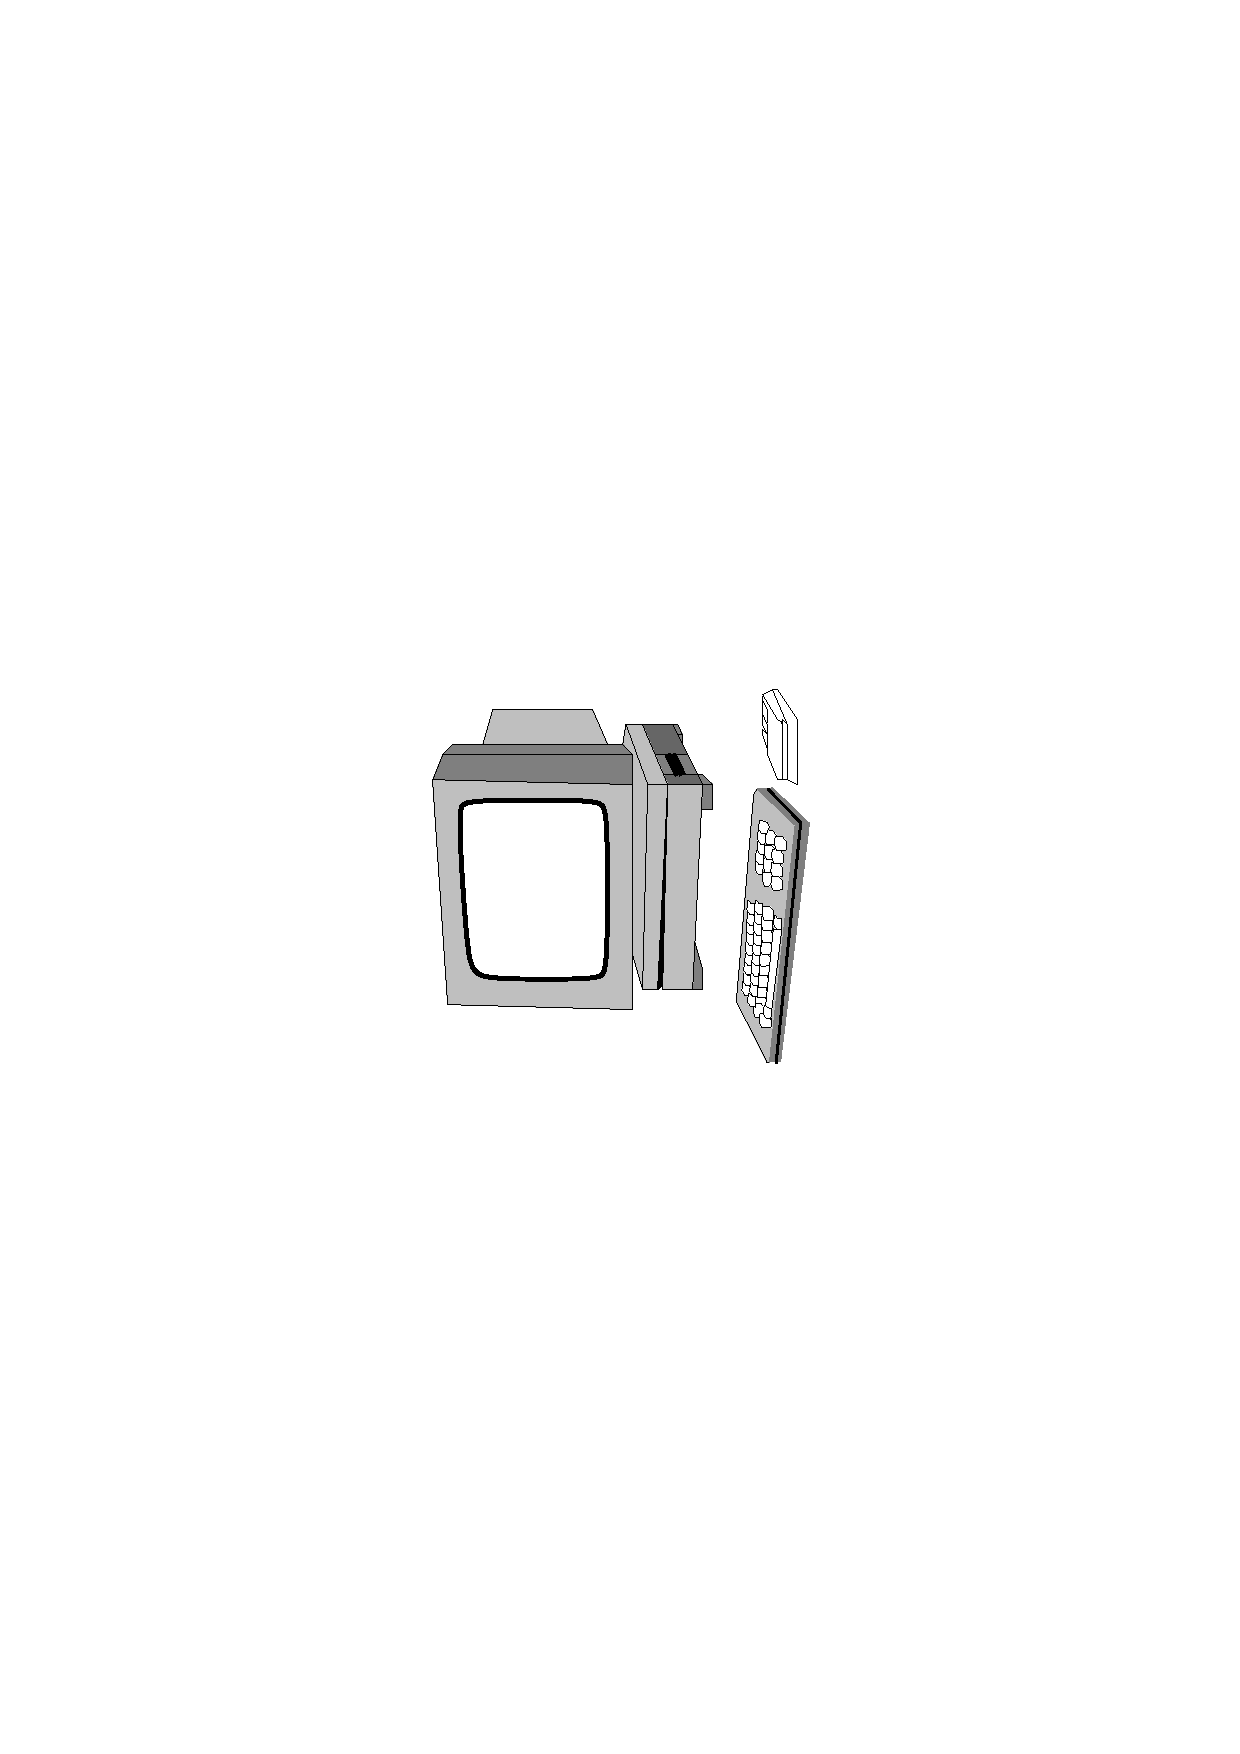
\includegraphics[width=4cm]{images/esempio}
   \caption{Esempio di figura\label{miafigura}}
   \end{figure}

\section{Equazioni}
   Le equazioni sono facilmente ottenibili, per esempio
   osservate nel sorgente $f(x)=x^{2}_{ij}\times \frac{(x+2)}{4}$
   oppure il suo equivalente~\ref{myeq} ottenuto utilizzando l'ambiente
   \emph{equation}:

   \begin{equation}
   \lim_{n \to \infty}
   \sum_{k=1}^n \frac{1}{k^2}
   = \frac{\pi^2}{6}
   \label{myeq}
   \end{equation}

\section{Lettere accentate\label{accenti}}

   Il \LaTeX2\/
   le gestisce benissimo: àèìòùÀÈÌÒÙáéíóúÁÉÍÓÚ (se avete l'accortezza di salvare i file con codifica \texttt{UTF-8}
   ma le nostre tastiere un po' meno\footnote{in realt\`a a volte l'ALT di destra
   usato con la vocale opportuna o il tasto sopra/sottostante (con eventualmente lo
   shift per le maiuscole) produce i vari tipi di accento (acuto, ottuso, dieresi\ldots).},
   allora in questo caso si usa:
   \`a\`e\`{\i}\`o\`u\`A\`E\aa\v e e cos\`{\i} via...
   \newpage
   Comunque per avere maggiori informazioni leggetevi la guida \emph{The Not So Short Introduction to \LaTeX2}
   che trovate già stampata da qualche parte nei laboratori.

\chapter{La Bibliografia}

   Per la gestione semplice e intuitiva della bibliografia si usa un programma
   aggiuntivo, il \BibTeX. A tal fine provate a dare il comando
   \texttt{bibtex tesi} e poi ri-latexxare due volte\footnote{se non funziona
   probabilmente non vi siete copiati i file local.bib e public.bib.}.
   Usando xdvi potrete notare che \`e stata completata la bibliografia
   e inserite le seguenti citazioni~\cite{sql,cv1,itsc99,mpi-boselli,mpipov,isata99,spie99,ipps99,iv98-1,iv98-2,spie98,isata97,iv97,camp97,canpc,ica3pp97,eusipco96,iv96,icip96}

   Per capire come \`e stato ottenuto il tutto guardate il sorgente, 
   provate poi ad osservare i file .bib per capire come aggiungere materiale da
   citare (il tutto \`e comunque spiegato in~\cite{btxdoc})\footnote{In realt\`a
   \`e decisamente conveniente includere file di bibliografie gi\`a esistenti.
   Per esempio,
   la maggioranza di voi hanno gi\`a definita una variabile BIBINPUTS che punta, tra le altre cose, ad
   alcune directory dove esistono alcuni file .bib che \`e gi\`a possible
   includere. Sicuramente il vostro co/relatore ha una directory in cui sono contenuti
   uno o pi\`u file .bib con le citazioni che fanno al vostro caso, fatevela dire
   e modificate la variabile di ambiente BIBINPUTS (nel file .user-cshrc) aggiungendo
   il \emph{path} opportuno.}

   Dal nostro sito web (area studenti) è possibile scaricarsi il database in formato \BibTeX di
   tutte le tesi sperimentali dal 1990 ai giorni nostri.



